\documentclass{article}   	                         % use "amsart" instead of "article" for AMSLaTeX format
\usepackage{fullpage}                		% ... or a4paper or a5paper or ... 
\usepackage{enumerate}				% Use enumerate to list subsections
\usepackage{graphicx}				% Use pdf, png, jpg, or eps§ with pdflatex; use eps in DVI mode
\usepackage{fancyvrb}
\usepackage{amsmath}
\usepackage{dsfont}
\newcommand{\ra}{\rightarrow}

%SetFonts

\title{Computer System Fundamentals HW \#4}
\author{Quan Zhou}
\date{Feb 18th, 2016}
\begin{document}
\maketitle
\section*{Problem 1}
\begin{enumerate}[(a)]
\item
Since the streaming media buffer system has:
\begin{enumerate}[.]
\item Arrival of the packets to the application follows Poisson process;
\item The processing time for each packet is an exponentially distributed variable;
\item Only one server processing;
\item The buffer can hold up to K packets, or the system size is finite;
\end{enumerate}
we can model the above system as an M/M/1/K system.\\
\item
$\rho = \lambda T_s = (50 \text{  packets per second})(20 \text {  msec}) = (50 \text{  packets per second})(0.02 \text {  sec}) = 1 \text {  packet}$\\
Since $\rho = 1$, $q = \frac{K}{2}  = 1.5$\\
\item
$\text {Pr}(S_K) = \frac{1}{K+1} = \frac{1}{4}$\\
$\text {Pr}(\bar S_K) = 1 - \frac{1}{K+1} = \frac{3}{4}$\\
so out of 2000 packets, there are 500 blips and 1500 plops.\\
\item
$$T_q = \frac{q}{\lambda \prime} = \frac{q}{\lambda (1-\text{Pr}(S_k))} = \frac{1.5}{0.05 \text{  packets per msec} (1 - \frac{1}{4})} = 40 \text{  msec}$$
\item
If K = 10:\\
$$q = \frac{K}{2} = 5$$
$$\text {Pr}(S_K) = \frac{1}{K+1} = \frac{1}{11}$$
$$T_q \prime = \frac{q}{\lambda \prime} = \frac{q}{\lambda (1-\text{Pr}(S_k \prime))} = \frac{5}{0.05 \text{  packets per msec} (1 - \frac{1}{11})} = 110 \text{  msec}$$
\item
As K increases, the buffer system size increases so that more packets are likely to be plopped in the played out and waited in the queue. So the mean response time/delay time for the packet from arrival to being serviced increases.\\
In general, the mean delay for packets that are played out to increase.
\item
\begin{BVerbatim}
"Increasing the size of network buffers (i.e., K) has its advantages and its disadvantages".
\end{BVerbatim}
\\
clearly the advantage of larger size of network buffer is less blips and more plops; but the disadvantage is the mean delay increases and resulting in an extended buffering process.\\ 
\item
For "Movie on Demand" streaming application like Netflix, larger buffer size (or larger K) is preferred because we do not want to have dropped the video data packets (or blips) making the video not watchable. It is OK for delay time to be increased as long as the quality of video is not compromised.\\
For teleconferencing application like Skype, smaller buffer size would be more preferable because even though blips could affect the voice data being transferred the audiences could still catch the meaning thus making the audio understandable. In cases like this having longer delay is bad because it delays the communication. In general, it is better to hear something immediately than nothing for a while.\\ 
\end{enumerate}

\section*{Problem 2}
\begin{enumerate}[(a)]
\item
Base on the results from $\text {sim1 log.txt}$, we imported the data into Excel and analyzed column Tq, and q (which is calculated from $\lambda T_q$). We found the mean $\mu$ and standard deviation $s$ to be (0.039, 0.032) sec and q (3.13 , 1.59) requests.\\
Assuming the data being normal and use the formula below to find confidence interval:\\
\begin{equation} \left[\bar X - z\frac{\sigma}{\sqrt n}, \bar X + z\frac{\sigma}{\sqrt n}\right]\end{equation}
so the confidence level for q is $[0.008, 6.24]$ and $T_q$ $[-0.023, 0.102]$\\
Compared to :\\
$$\rho = \lambda Ts = 50*0.02 = 1$$
$$q = \frac{K}{2} = 3/2 = 1.5$$
$$w = q-\rho = 1.5 - 1 = 0.5 $$
$$T_q = \frac{q}{\lambda} = \frac{1.5}{50} = 0.03$$
$$T_w = \frac{w}{\lambda} = \frac{0.5}{50} = 0.01$$
$$\text {Pr ("Rejection")} = \frac{1}{K+1} = 0.25 $$
We found $1.5$ falls in the $95\%$ confidence interval $[0.008, 6.24]$ for q and $ 0.03$ in $[-0.023, 0.102]$ for $T_q$.\\

\item
Base on the results from $\text {sim2 log.txt}$, we imported the data into Excel and analyzed column Tq, and q (which is calculated from $\lambda T_q$). We found the mean $\mu$ and standard deviation $s$ to be (0.028, 0.024) sec and q (1.406 , 1.206) requests.\\
Using equation from part (a), we calculate the $95\%$ confidence level for q is $[0, 3.77]$ and $T_q$ $[-0.019, 0.072]$\\
Compared to :\\
$$\rho = \lambda Ts = 50*0.015 = 0.75$$
$$q = \frac{\rho}{1-\rho} - \frac{(K+1)\rho^{K+1}}{1-\rho^{K+1}} = 3 - \frac{4 0.75^4}{1-0.75^4} = 1.15$$
$$w = q-\rho = 1.15 - 0.75 = 0.4 $$
$$T_q = \frac{q}{\lambda} = \frac{1.15}{50} = 0.023$$
$$T_w = \frac{w}{\lambda} = \frac{0.4}{50} = 0.008$$
$$\text {Pr ("Rejection")} = \frac{(1-\rho)\rho^K}{1-\rho^{K+1}} = \frac{(0.25)0.75^3}{1-0.75^4} = 0.1542  $$
We found $1.15$ falls in the $95\%$ confidence interval $[0, 3.77]$ for q and $ 0.023$ in $[-0.019, 0.072]$ for $T_q$.\\

\item
Base on the results from $\text {sim3 log.txt}$, we imported the data into Excel and analyzed column Tq, and q (which is calculated from $\lambda T_q$). We found the mean $\mu$ and standard deviation $s$ to be (0.030, 0.024) sec and q (1.963 , 1.589) requests.\\
so the confidence level for q is $[0, 5.078]$ and $T_q$ $[-0.018, 0.078]$\\
Compared to :\\
$$\rho = \lambda Ts = 65*0.015 = 0.975$$
$$q = \frac{\rho}{1-\rho} - \frac{(K+1)\rho^{K+1}}{1-\rho^{K+1}} = 39 - \frac{4 0.975^4}{1-0.975^4} = 1.468$$
$$w = q-\rho = 1.468 - 0.975 = 0.493 $$
$$T_q = \frac{q}{\lambda} = \frac{1.468}{65} = 0.0226$$
$$T_w = \frac{w}{\lambda} = \frac{0.493}{65} = 0.0076$$
$$\text {Pr ("Rejection")} = \frac{(1-\rho)\rho^K}{1-\rho^{K+1}} = \frac{(0.025)0.975^3}{1-0.975^4} = 0.2346 $$
We found $1.468$ falls in the $95\%$ confidence interval $[0, 5.078]$ for q and $ 0.0226$ in $[-0.018, 0.078]$ for $T_q$.\\

\item
Base on the results from $\text {sim4 log.txt}$, we imported the data into Excel and analyzed column Tq, and q (which is calculated from $\lambda T_q$). We found the mean $\mu$ and standard deviation $s$ to be (0.024, 0.009) sec and q (1.561 , 0.610) requests.\\
so the confidence level for q is $[0.364, 2.757]$ and $T_q$ $[0.006, 0.042]$\\
Compared to the confidence level for q is $[0.008, 6.24]$ and $T_q$ $[-0.023, 0.102]$ found in part (a):\\
Because of the huge variation from the run in part a, it is unclear if the rejection probability varied because of the change in the distribution of service time. But intuitively, the rejection probability given this M/D/1/K system should be LESS: Since the utilization for part (d) is less than that of part (a), it is less likely for the system in (d) to reject a process because it has higher change of idle time.

\item
Base on the results from $\text {sim5 log.txt}$, we imported the data into Excel and analyzed column Tq, and q (which is calculated from $\lambda T_q$). We found the mean $\mu$ and standard deviation $s$ to be (0.028, 0.010) sec and q (1.806 , 0.642) requests.\\
so the confidence level for q is $[0.547, 3.065]$ and $T_q$ $[0.008, 0.047]$\\
Compared to the confidence level for q $[0, 3.77]$ and $T_q$ $[-0.019, 0.072]$ from part (b):\\
Because of the huge variation from the run in part a, it is unclear if the rejection probability varied because of the change in the distribution of service time. But intuitively, the rejection probability given this M/D/1/K system at arrival rate being 65 should be MORE: Given all things equal, it is more likely for the system to reject an incoming process because it has higher rate 
\\
\\
\begin{BVerbatim}
Results from M/M/1 system in Assignment 3:
\end{BVerbatim}
\begin{enumerate}
\item part b (HW3) versus part b (HW4)\\
Given the same settings: $\lambda = 50$, $T_s = 0.015$, and Simulation time is 100, M/M/1 and M/M/1/K behaves somewhat similar. As we calculated the $\rho$ to be 0.75, which resulted $q = 3$ for M/M/1 system. In a way it behaves like the M/M/1/K system with the queue size of 3. and turns out the mean value of q and $T_q$ are about the same.
\item part c (HW3) versus part c (HW4)\\
Though the settings ($\lambda = 65$, $T_s = 0.015$, and Simulation time is 100), M/M/1 system without buffer limit was able to surpass that of M/M/1/K with $K = 3$. In M/M/1, mean value of q is about 40 empirically (analytically too be 39) where as in M/M/1/K (K = 3) is only 1.15. These makes sense as it shows how much the queue size limits the performance of the server even though utilization is high.\\

\end{enumerate}
\begin{BVerbatim}
NOTE:\\
\end{BVerbatim}
All the log files were printed from the console, copied in these txt files and then imported in excel. Due to time constraints, I was not able to generate auto-log and auto-import codes for M/M/1/K and M/D/1/K simulations.\\

\end{enumerate}

\section*{Problem 3}
\begin{enumerate}[(a)]
\item
Recall the diagram from HW3:\\
\begin{center}
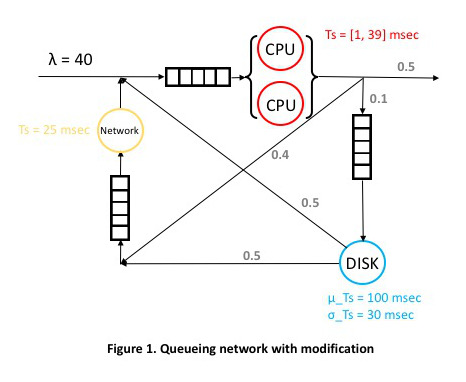
\includegraphics[scale = 0.5]{Figure1.jpg}
\end{center}
We have modified the computation based on problem 3 and ran the java code (courtesy to Auwong) and obtained a log of the simulation:\\
Final Results of simulation: \\
$T_w$: 0.5424771197409428\\
$T_q$: 0.563099166123886\\
$w_{cpu}$: 1.5454545454545454\\
$q_{cpu}$: 3.164869029275809\\
$w_{disk}$: 3.6512583461736003\\
$q_{disk}$: 4.49306625577812\\
$w_{net}$: 12.676938880328711\\
$q_{net}$: 13.622496147919877\\
\\	
Due to large quantity of data, was only able to print the last few seconds (assume the unit of time is second) out of 100 (See Figure 2).\\
\begin{center}
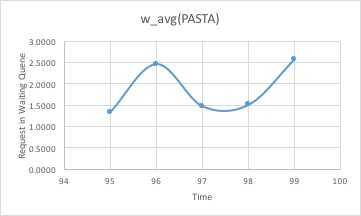
\includegraphics[scale = 0.5]{Figure2.jpg}
\end{center}

\item
The system may reach the steady state long before the last few seconds, but i am confident that this CPU/DISK/network system has reached steady state by the end of 100 seconds.\\
\item
The Z-scores for $95\%$ and $98\%$ are 1.96 and 2.32 respectively. I calculated the confidence interval in the code (see LogEvent.java) and obtained the following:\\
\begin{BVerbatim}
95% Confidence Interval:
\end{BVerbatim}
\\
For q: [3.1659-5.5996, 3.1659+5.5996]\\ 
For Tq: [0.5631-1.4925, 0.5631+1.4925]\\
\\
\begin{BVerbatim}
98% Confidence Interval:
\end{BVerbatim}
\\
For q: [3.1659-6.6281, 3.1659+6.6281]\\ 
For Tq: [0.5631-1.7667, 0.5631+1.7667]\\
\\
The simulation somehow has large variation for the values above. 
\item
From HW3, I calculated the following metrics below:\\
\begin{equation}x = 0.5x + 40\end{equation}
so $x = 80\text {   processes per second}$ = 0.08\text {   processes per msec}.\\
Now we can find:\\
\begin{align*}
  \rho_{CPU} &= \frac{1}{2}\lambda_{CPU}T_s(CPU) = \frac{1}{2}(0.08)(20) = 0.8 (versus \frac{1}{2} *(3.1649-1.5454) = 0.8097)\\
  \rho_{DISK} &= \lambda_{DISK}T_s(DISK) = (0.1)(0.08)(100) = 0.8 (versus 4.4931- 3.6513 = 0.8418)\\
  \rho_{Network} &= \lambda_{Network}T_s(Network) = [(0.4)(0.08) + (0.1)(0.08)(0.5)](25) = 0.9 (versus 13.6225- 12.6769= 0.9456)\\
q_{CPU} &= \frac{\rho_{CPU}}{1-\rho_{CPU}} = 4 (versus 3.16)\\
q_{DISK} &= 4 (versus 4.49) \\
q_{Network} & = 9 (versus 13.62)
\end{align*} 
So simulation results make sense and are very close to the analytical results \\
\begin{BVerbatim}
NOTE: parentheses are the simulation results\\
\end{BVerbatim}
\end{enumerate}

\section*{Problem 4}
\begin{enumerate}[(a)]
\item
When I modified $\lambda$ to 1 request per second, i obtained the following results:\\
98th Confidence level E = 0.036675890831936536\\
98th Confidence level E = 0.0288449709524687\\
Final Results of simulation: \\
	$T_w$: 0.044206714195278024\\
	$T_q$: 0.05780577574711234\\
	$w_{cpu}$: 0.0\\
	$q_{cpu}$: 0.018867924528301886\\
	$w_{disk}$: 0.0\\
	$q_{disk}$: 0.018867924528301886\\
	$w_{net}$: 0.0\\
	$q_{net}$: 0.018867924528301886\\
	95 $\%$ Confidence level of q: [0.01887-0.0310, 0.01887+0.0310]\\
	95 $\%$ Confidence level of Tq: [0.0578-0.0244, 0.0578+0.0244]\\
Therefore, the slowdown of the system ($\lambda = 40$) is :\\
$$\text{ Slowdown} = \frac{T_q}{T_s} = \frac{T_q (\lambda=40}{T_q (\lambda\rightarrow 1} = \frac{0.5631}{0.0578}= 9.74$$
\item
From the calculations in HW3, it is known that the network is the bottleneck for it would hit 100$\%$ utilization first.  Let the rate going through CPU be x processes per second. I have the following flowrate balance for Network server:\\
$$[0.4(x) + 0.1(x) (0.5)]25 = 1$$
so x is found to be $\frac{4}{45}$ or 0.088 requests per msec, which is our upper limit of $\lambda$.\\
I collected the simulation results given $\lambda$ in the range from 1 to 70 requests/msec (Table 1) and then plotted the utilization of all three serving units in this system. 
\begin{center}
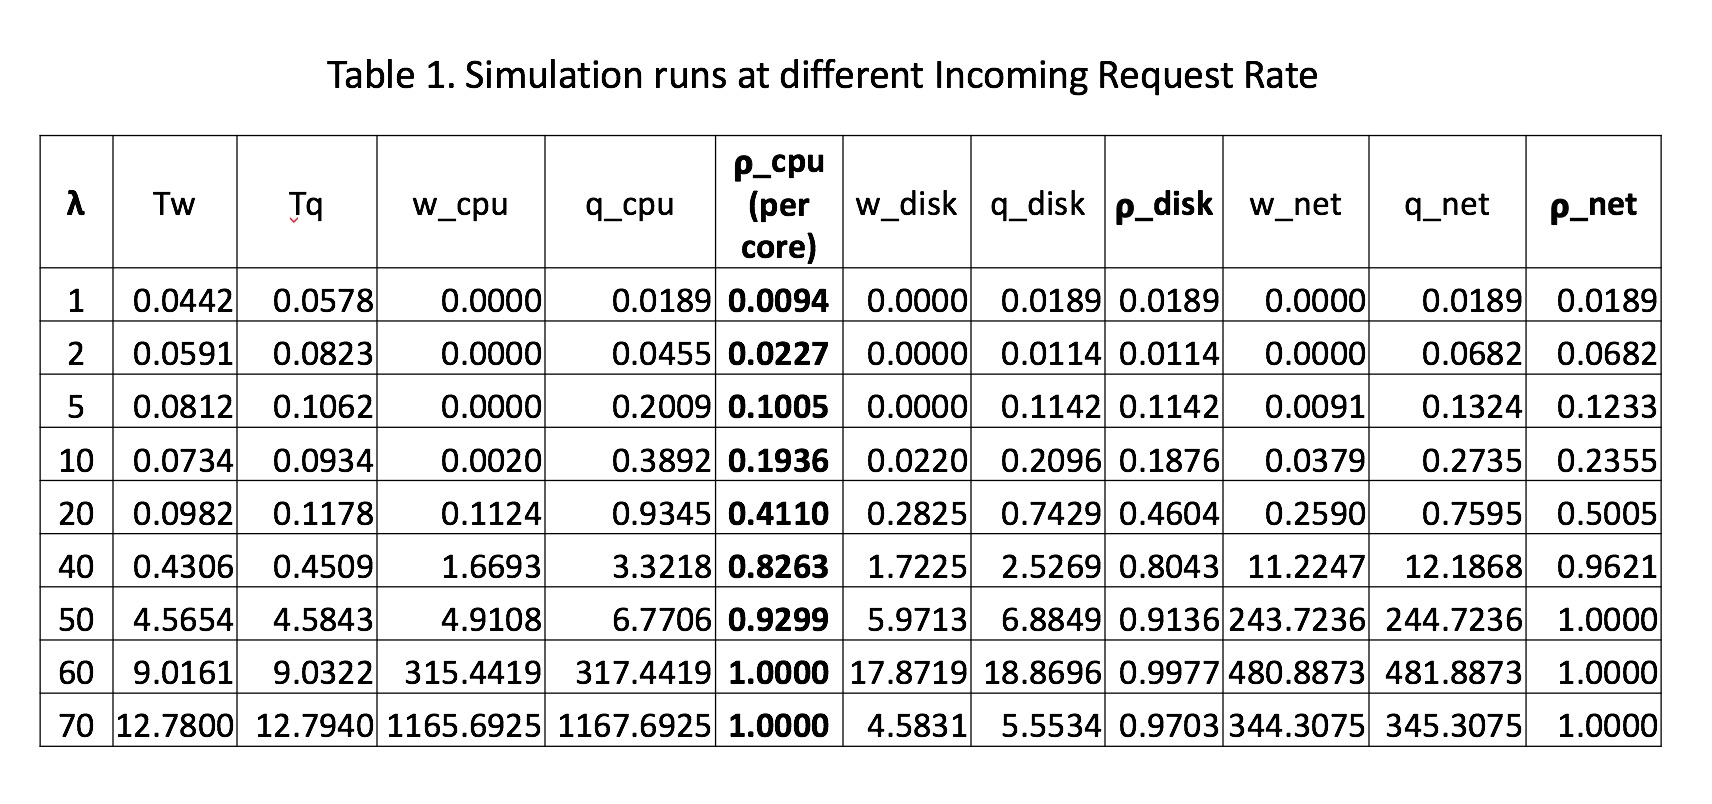
\includegraphics[scale = 0.2]{Figure3.jpg}
\end{center}
The simulation agrees with the analytical results in which the network server hits $100\%$ utilization first but at $\lambda = 50$.
\begin{center}
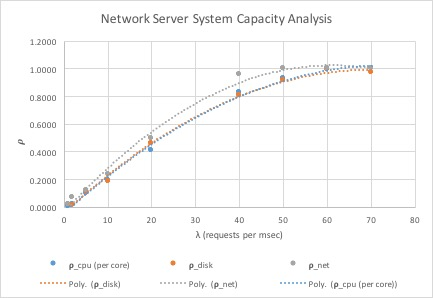
\includegraphics[scale = 0.8]{Figure4.jpg}
\end{center}
 
\end{enumerate}

\end{document}